\documentclass[a4paper,12pt]{article}
\usepackage[utf8]{inputenc}
\usepackage[margin=1in]{geometry}
\usepackage{tikz}
\usepackage{xcolor}
\usetikzlibrary{shapes,arrows.meta,positioning,fit,backgrounds}

\definecolor{csvcolor}{RGB}{255,193,7}
\definecolor{pythoncolor}{RGB}{76,175,80}
\definecolor{owlcolor}{RGB}{33,150,243}
\definecolor{ttlcolor}{RGB}{156,39,176}
\definecolor{graphdbcolor}{RGB}{244,67,54}
\definecolor{webcolor}{RGB}{0,188,212}

\title{\textbf{PKG2020 Knowledge Graph Pipeline}}
\author{KRR Project - Data Conversion Workflow}
\date{}

\begin{document}

\maketitle

\section*{Overview}
This document shows the complete pipeline for converting raw CSV data into a semantic knowledge graph with SPARQL endpoint and web visualization.

\vspace{1cm}

\begin{center}
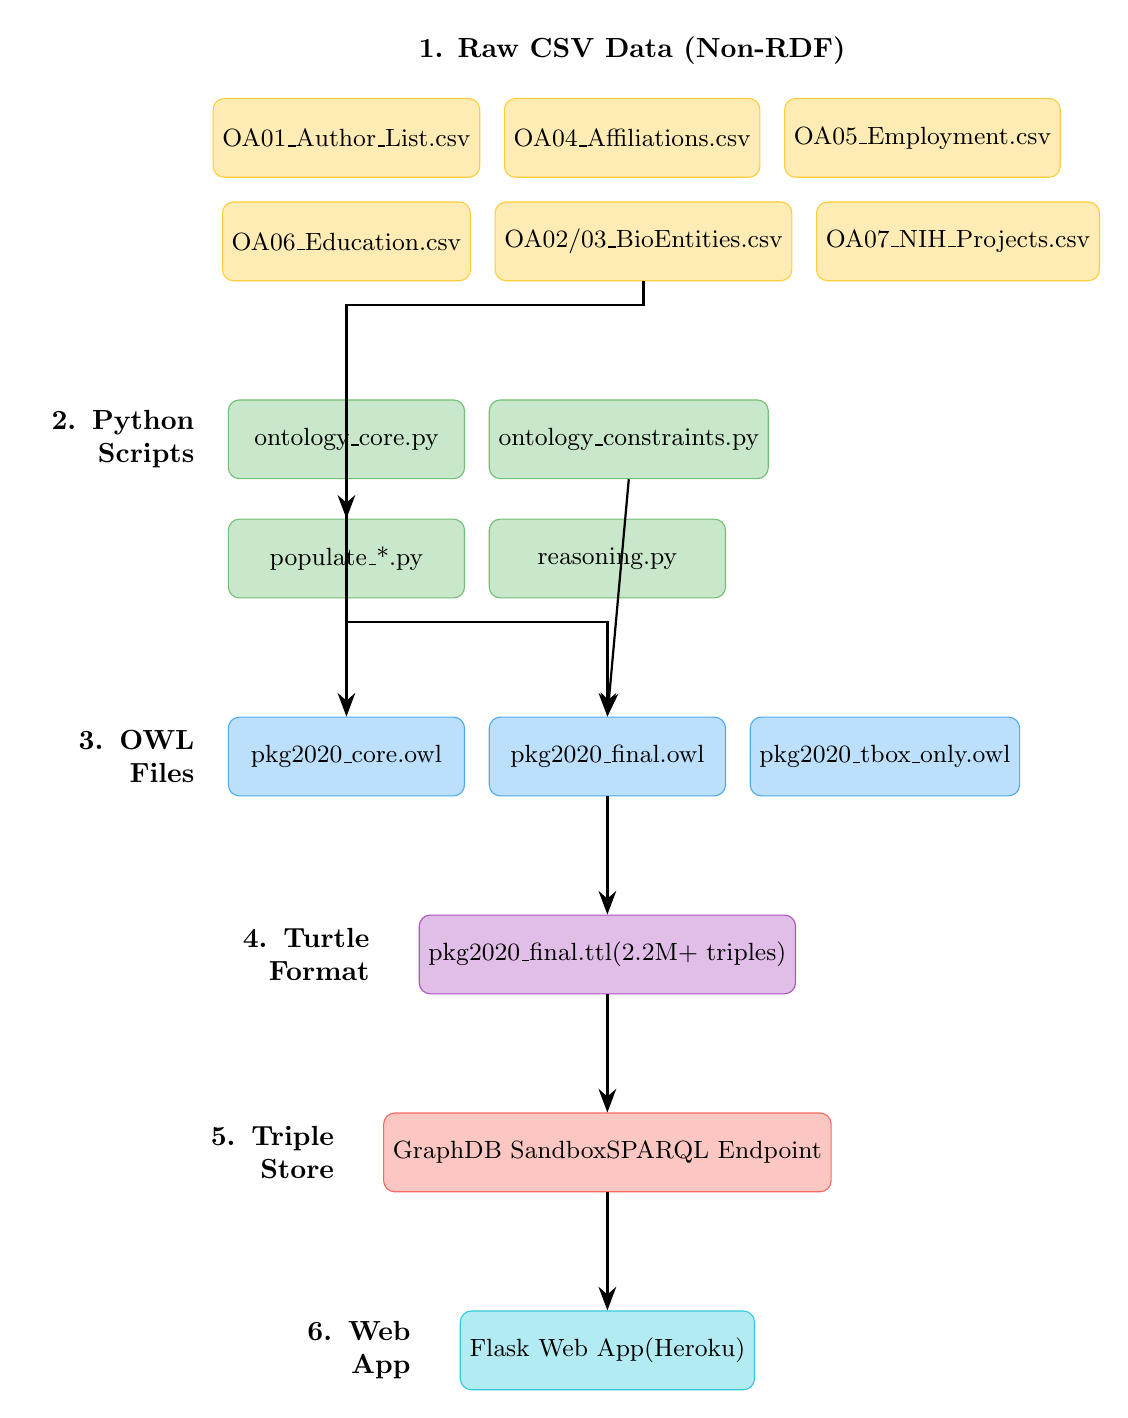
\begin{tikzpicture}[
    node distance=0.8cm,
    box/.style={rectangle, draw, rounded corners, minimum width=3cm, minimum height=1cm, text centered, font=\small},
    csv/.style={box, fill=csvcolor!30, draw=csvcolor!80},
    python/.style={box, fill=pythoncolor!30, draw=pythoncolor!80},
    owl/.style={box, fill=owlcolor!30, draw=owlcolor!80},
    ttl/.style={box, fill=ttlcolor!30, draw=ttlcolor!80},
    graphdb/.style={box, fill=graphdbcolor!30, draw=graphdbcolor!80},
    web/.style={box, fill=webcolor!30, draw=webcolor!80},
    arrow/.style={-{Stealth[length=3mm]}, thick}
]

% Row 1: CSV Files
\node[csv] (csv1) {OA01\_Author\_List.csv};
\node[csv, right=0.3cm of csv1] (csv2) {OA04\_Affiliations.csv};
\node[csv, right=0.3cm of csv2] (csv3) {OA05\_Employment.csv};
\node[csv, below=0.3cm of csv1] (csv4) {OA06\_Education.csv};
\node[csv, right=0.3cm of csv4] (csv5) {OA02/03\_BioEntities.csv};
\node[csv, right=0.3cm of csv5] (csv6) {OA07\_NIH\_Projects.csv};

% Label for CSV
\node[above=0.3cm of csv2, font=\bfseries] {1. Raw CSV Data (Non-RDF)};

% Python Scripts
\node[python, below=1.5cm of csv4] (ontcore) {ontology\_core.py};
\node[python, right=0.3cm of ontcore] (ontcons) {ontology\_constraints.py};
\node[python, below=0.5cm of ontcore] (pop1) {populate\_*.py};
\node[python, right=0.3cm of pop1] (reason) {reasoning.py};

% Label for Python
\node[left=0.3cm of ontcore, font=\bfseries, text width=2cm, align=right] {2. Python Scripts};

% OWL Files
\node[owl, below=1.5cm of pop1] (owlcore) {pkg2020\_core.owl};
\node[owl, right=0.3cm of owlcore] (owlfinal) {pkg2020\_final.owl};
\node[owl, right=0.3cm of owlfinal] (owltbox) {pkg2020\_tbox\_only.owl};

% Label for OWL
\node[left=0.3cm of owlcore, font=\bfseries, text width=2cm, align=right] {3. OWL Files};

% TTL File
\node[ttl, below=1.5cm of owlfinal] (ttl) {pkg2020\_final.ttl\\(2.2M+ triples)};

% Label for TTL
\node[left=0.5cm of ttl, font=\bfseries, text width=2cm, align=right] {4. Turtle Format};

% GraphDB
\node[graphdb, below=1.5cm of ttl] (graphdb) {GraphDB Sandbox\\SPARQL Endpoint};

% Label for GraphDB
\node[left=0.5cm of graphdb, font=\bfseries, text width=2cm, align=right] {5. Triple Store};

% Web App
\node[web, below=1.5cm of graphdb] (webapp) {Flask Web App\\(Heroku)};

% Label for Web
\node[left=0.5cm of webapp, font=\bfseries, text width=2cm, align=right] {6. Web App};

% Arrows
\draw[arrow] (csv5.south) -- ++(0,-0.3) -| (pop1.north);
\draw[arrow] (ontcore.south) -- (owlcore.north);
\draw[arrow] (ontcons.south) -- (owlfinal.north);
\draw[arrow] (pop1.south) -- ++(0,-0.3) -| (owlfinal.north);
\draw[arrow] (owlfinal.south) -- (ttl.north);
\draw[arrow] (ttl.south) -- (graphdb.north);
\draw[arrow] (graphdb.south) -- (webapp.north);

\end{tikzpicture}
\end{center}

\newpage

\section*{Pipeline Steps - Detailed}

\subsection*{Step 1: Raw CSV Data $\rightarrow$ Python Processing}
\begin{center}
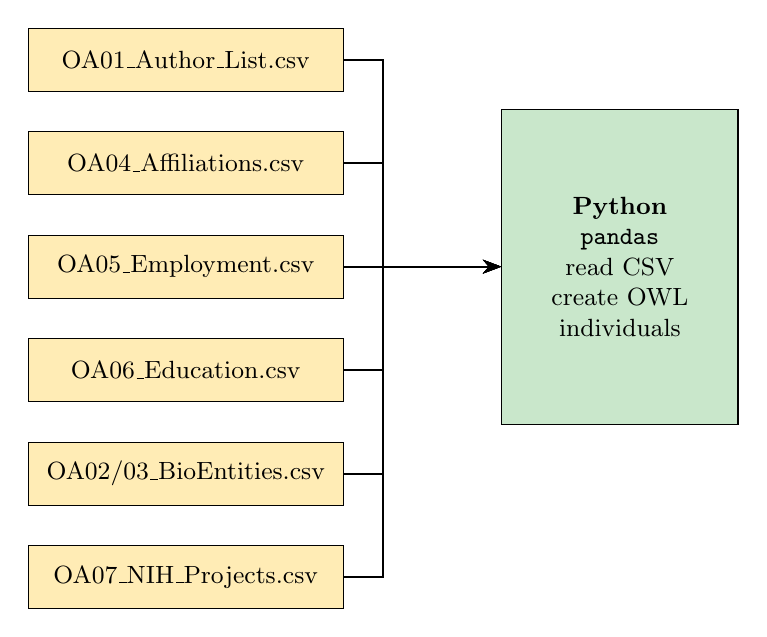
\begin{tikzpicture}[
    node distance=0.5cm,
    file/.style={rectangle, draw, fill=csvcolor!30, minimum width=4cm, minimum height=0.8cm, font=\small},
    arrow/.style={-{Stealth}, thick}
]
\node[file] (a) {OA01\_Author\_List.csv};
\node[file, below=of a] (b) {OA04\_Affiliations.csv};
\node[file, below=of b] (c) {OA05\_Employment.csv};
\node[file, below=of c] (d) {OA06\_Education.csv};
\node[file, below=of d] (e) {OA02/03\_BioEntities.csv};
\node[file, below=of e] (f) {OA07\_NIH\_Projects.csv};

\node[right=2cm of c, rectangle, draw, fill=pythoncolor!30, minimum width=3cm, minimum height=4cm, font=\small, text width=2.5cm, align=center] (py) {\textbf{Python}\\\texttt{pandas}\\read CSV\\create OWL\\individuals};

\draw[arrow] (a.east) -- ++(0.5,0) |- (py.west);
\draw[arrow] (b.east) -- ++(0.5,0) |- (py.west);
\draw[arrow] (c.east) -- (py.west);
\draw[arrow] (d.east) -- ++(0.5,0) |- (py.west);
\draw[arrow] (e.east) -- ++(0.5,0) |- (py.west);
\draw[arrow] (f.east) -- ++(0.5,0) |- (py.west);
\end{tikzpicture}
\end{center}

\subsection*{Step 2: Python Scripts Execution Order}
\begin{center}
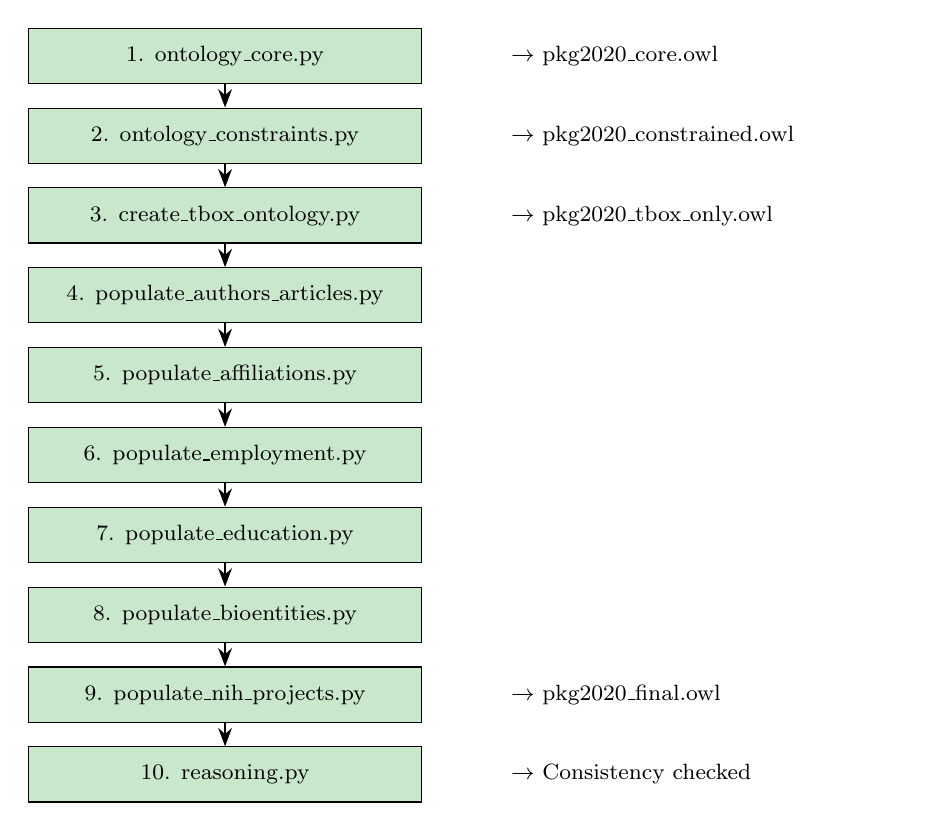
\begin{tikzpicture}[
    node distance=0.3cm,
    script/.style={rectangle, draw, fill=pythoncolor!30, minimum width=5cm, minimum height=0.7cm, font=\footnotesize},
    arrow/.style={-{Stealth}, thick}
]
\node[script] (s1) {1. ontology\_core.py};
\node[script, below=of s1] (s2) {2. ontology\_constraints.py};
\node[script, below=of s2] (s3) {3. create\_tbox\_ontology.py};
\node[script, below=of s3] (s4) {4. populate\_authors\_articles.py};
\node[script, below=of s4] (s5) {5. populate\_affiliations.py};
\node[script, below=of s5] (s6) {6. populate\_employment.py};
\node[script, below=of s6] (s7) {7. populate\_education.py};
\node[script, below=of s7] (s8) {8. populate\_bioentities.py};
\node[script, below=of s8] (s9) {9. populate\_nih\_projects.py};
\node[script, below=of s9] (s10) {10. reasoning.py};

\draw[arrow] (s1) -- (s2);
\draw[arrow] (s2) -- (s3);
\draw[arrow] (s3) -- (s4);
\draw[arrow] (s4) -- (s5);
\draw[arrow] (s5) -- (s6);
\draw[arrow] (s6) -- (s7);
\draw[arrow] (s7) -- (s8);
\draw[arrow] (s8) -- (s9);
\draw[arrow] (s9) -- (s10);

\node[right=1cm of s1, font=\footnotesize, text width=5cm] {$\rightarrow$ pkg2020\_core.owl};
\node[right=1cm of s2, font=\footnotesize, text width=5cm] {$\rightarrow$ pkg2020\_constrained.owl};
\node[right=1cm of s3, font=\footnotesize, text width=5cm] {$\rightarrow$ pkg2020\_tbox\_only.owl};
\node[right=1cm of s9, font=\footnotesize, text width=5cm] {$\rightarrow$ pkg2020\_final.owl};
\node[right=1cm of s10, font=\footnotesize, text width=5cm] {$\rightarrow$ Consistency checked};
\end{tikzpicture}
\end{center}

\subsection*{Step 3: OWL to Turtle Conversion}
\begin{center}
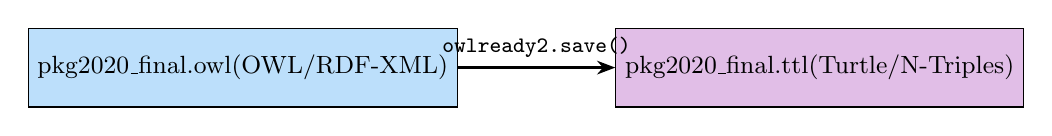
\begin{tikzpicture}[
    node distance=1.5cm,
    file/.style={rectangle, draw, minimum width=4cm, minimum height=1cm, font=\small},
    arrow/.style={-{Stealth}, thick, font=\footnotesize}
]
\node[file, fill=owlcolor!30] (owl) {pkg2020\_final.owl\\(OWL/RDF-XML)};
\node[file, right=2cm of owl, fill=ttlcolor!30] (ttl) {pkg2020\_final.ttl\\(Turtle/N-Triples)};

\draw[arrow] (owl) -- node[above] {\texttt{owlready2.save()}} (ttl);
\end{tikzpicture}
\end{center}

\subsection*{Step 4: Upload to GraphDB}
\begin{center}
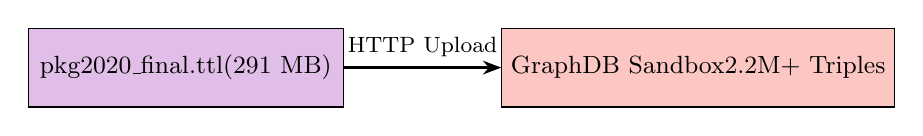
\begin{tikzpicture}[
    node distance=1.5cm,
    file/.style={rectangle, draw, minimum width=4cm, minimum height=1cm, font=\small},
    arrow/.style={-{Stealth}, thick}
]
\node[file, fill=ttlcolor!30] (ttl) {pkg2020\_final.ttl\\(291 MB)};
\node[file, right=2cm of ttl, fill=graphdbcolor!30] (gdb) {GraphDB Sandbox\\2.2M+ Triples};

\draw[arrow] (ttl) -- node[above, font=\footnotesize] {HTTP Upload} (gdb);
\end{tikzpicture}
\end{center}

\subsection*{Step 5: SPARQL Endpoint Access}
\begin{center}
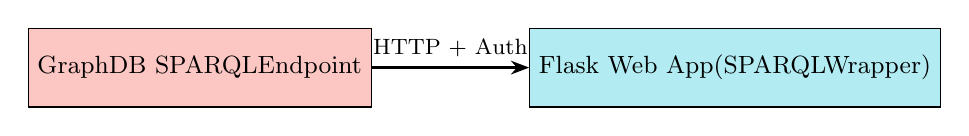
\begin{tikzpicture}[
    node distance=1.5cm,
    file/.style={rectangle, draw, minimum width=4cm, minimum height=1cm, font=\small},
    arrow/.style={-{Stealth}, thick}
]
\node[file, fill=graphdbcolor!30] (gdb) {GraphDB SPARQL\\Endpoint};
\node[file, right=2cm of gdb, fill=webcolor!30] (app) {Flask Web App\\(SPARQLWrapper)};

\draw[arrow] (gdb) -- node[above, font=\footnotesize] {HTTP + Auth} (app);
\end{tikzpicture}
\end{center}

\section*{Output Files Summary}

\begin{center}
\begin{tabular}{|l|l|l|}
\hline
\textbf{File} & \textbf{Purpose} & \textbf{Size} \\
\hline
pkg2020\_tbox\_only.owl & T-Box (schema only) & 14 KB \\
pkg2020\_hand\_annotated.owl & 10+ hand-annotated & 19 KB \\
pkg2020\_with\_swrl.owl & SWRL rules & 27 KB \\
pkg2020\_final.owl & Complete ontology & 119 MB \\
pkg2020\_final.ttl & Turtle for GraphDB & 291 MB \\
\hline
\end{tabular}
\end{center}

\section*{Technology Stack}

\begin{center}
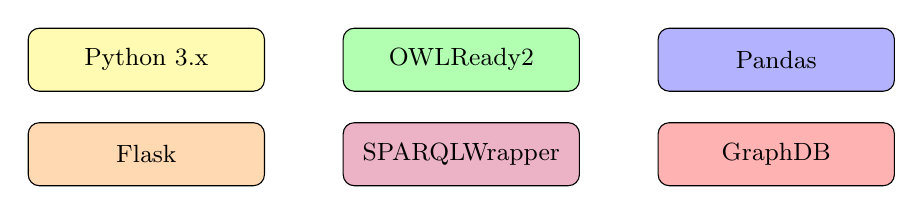
\begin{tikzpicture}[
    box/.style={rectangle, draw, rounded corners, minimum width=3cm, minimum height=0.8cm, text centered, font=\small}
]
\node[box, fill=yellow!30] at (0,0) {Python 3.x};
\node[box, fill=green!30] at (4,0) {OWLReady2};
\node[box, fill=blue!30] at (8,0) {Pandas};
\node[box, fill=orange!30] at (0,-1.2) {Flask};
\node[box, fill=purple!30] at (4,-1.2) {SPARQLWrapper};
\node[box, fill=red!30] at (8,-1.2) {GraphDB};
\end{tikzpicture}
\end{center}

\end{document}
